\section{Google Remote Procedure Call (gRPC)}
Der neue Standard-Technologie für die Backend-Kommunikation in .NET. Primär Server-to-Server Kommunikation im Fokus (Microservices). Hohe Performance von zentraler Bedeutung. Nicht als Frontend-API gedacht. Ist der Ersatz für Windows Communication Foundation. . Kommunikation über HTTP/2 (Multiplexing (mehrere gRPC Calls pro TCP/IP Connection), Bidirectionales Streaming, Parallele Requests und Responses in einer einzigen TCP Verbindung, Kommunikation wegen HTTPS verschlüsselt).

\begin{figure}[h!]
  	\centering
  	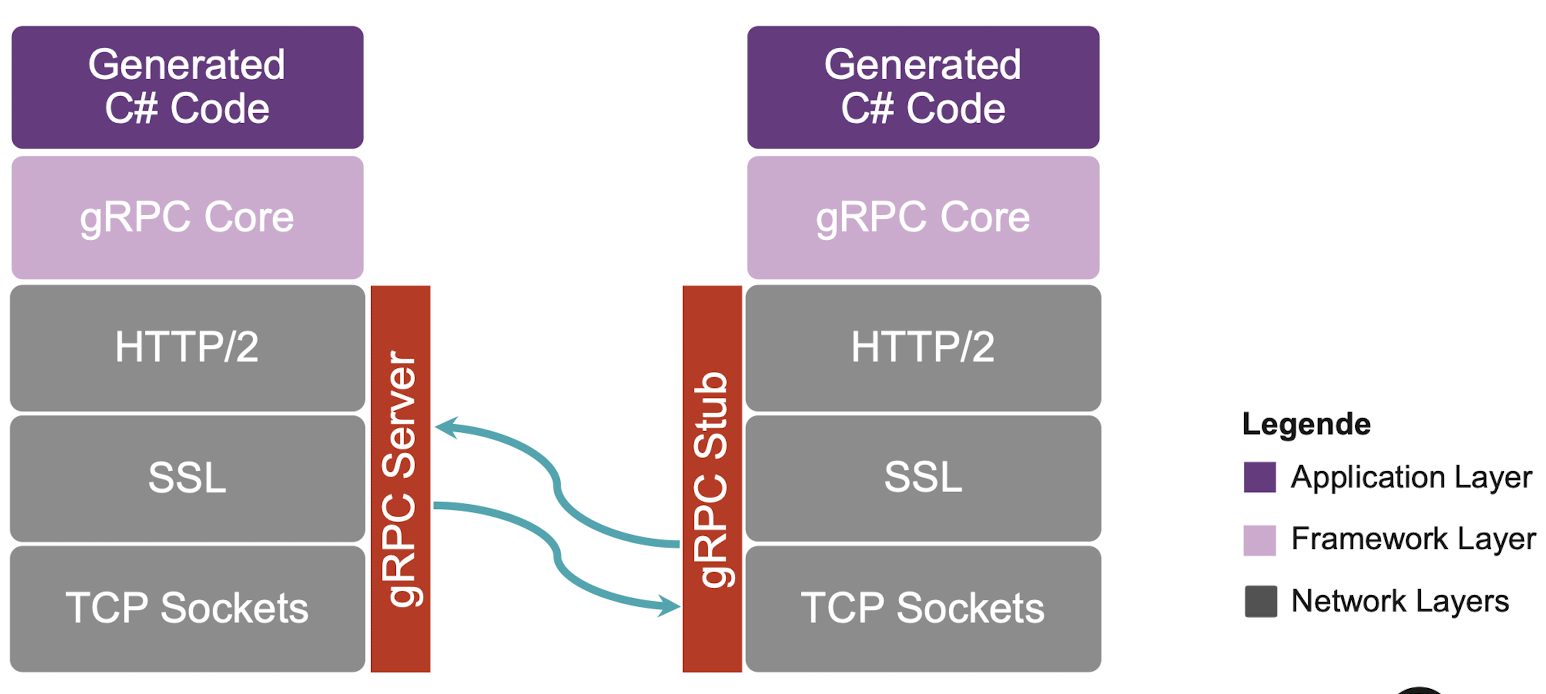
\includegraphics[width=0.5\linewidth]{communicationstack}
  \caption{Kommunikationsstack}
\end{figure}

\begin{description}
  \item[Kommunikationsprotokoll] HTTP/2
  \item[Interface Definition Language] Google Protocol Buffers
\end{description}

\subsection{Architektur}
gRPC ist ein SDK und kann in verschiedene IDEs integriert werden. 

\begin{figure}[h!]
	\centering
	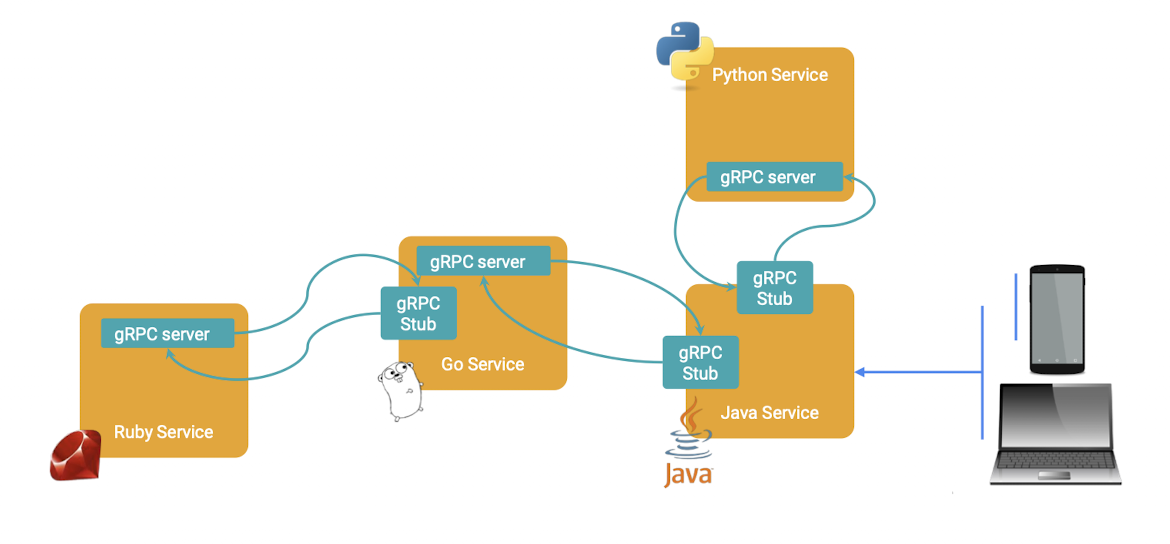
\includegraphics[width=0.75\linewidth]{gRPC}
 	\caption{Architekturbeispeil}
\end{figure}



\textbf{HTTP/2 Features}
\begin{description}
  \item[Multiplexing] Mehrere gRPC Calls pro TCP/IP Session
  \item[Bidirectional Streaming] Asynchronis, nicht-blockierendes Senden und Empfangen von Streams
  \item[HTTPS] HTTP/2 und gRPC basieren voll auf HTTPS $\rightarrow$ Kommunikation ist immer verschlüsselt
\end{description}

\subsection{Protocol Buffers}
\begin{itemize}
  \itemsep -0.5em 
  \item Interface Definition Language (IDL)
  	\SubItem{Ene Subform einer Domain Specific Language (DSL)}
  	\SubItem{Beschreibt ein Service Interface plattform- und sprachneutral.}
  \item Data Model
  	\SubItem{Beschreibt Messages resp. Request- und Response-Objekte}
  \item Wire Format
  	\SubItem{Beschreibt das Binärformat zu Übertragung}
  \item Seriealisierung- und Deserialisierungmechanismen
  \item Service-Versionierung
\end{itemize}

\textbf{Proto Files} \\
Datei-Endung "*.proto". Service-Methoden haben immer einen Parameter und einen Rückgabewert. 1 oder mehr Services und 1 oder mehr Service-Methoden pro Service. 1 oder mehr Message Type Fields. Service Methoden haben immer 1 Parameter und 1 Rückgabewert.

\textbf{Messages} \\
Angabe der Feldtypen: Skalarer Typ, Anderer Message Type, Enumeration. Unique Field Name und Unique Field Number.

\begin{figure}[h!]
  \center
  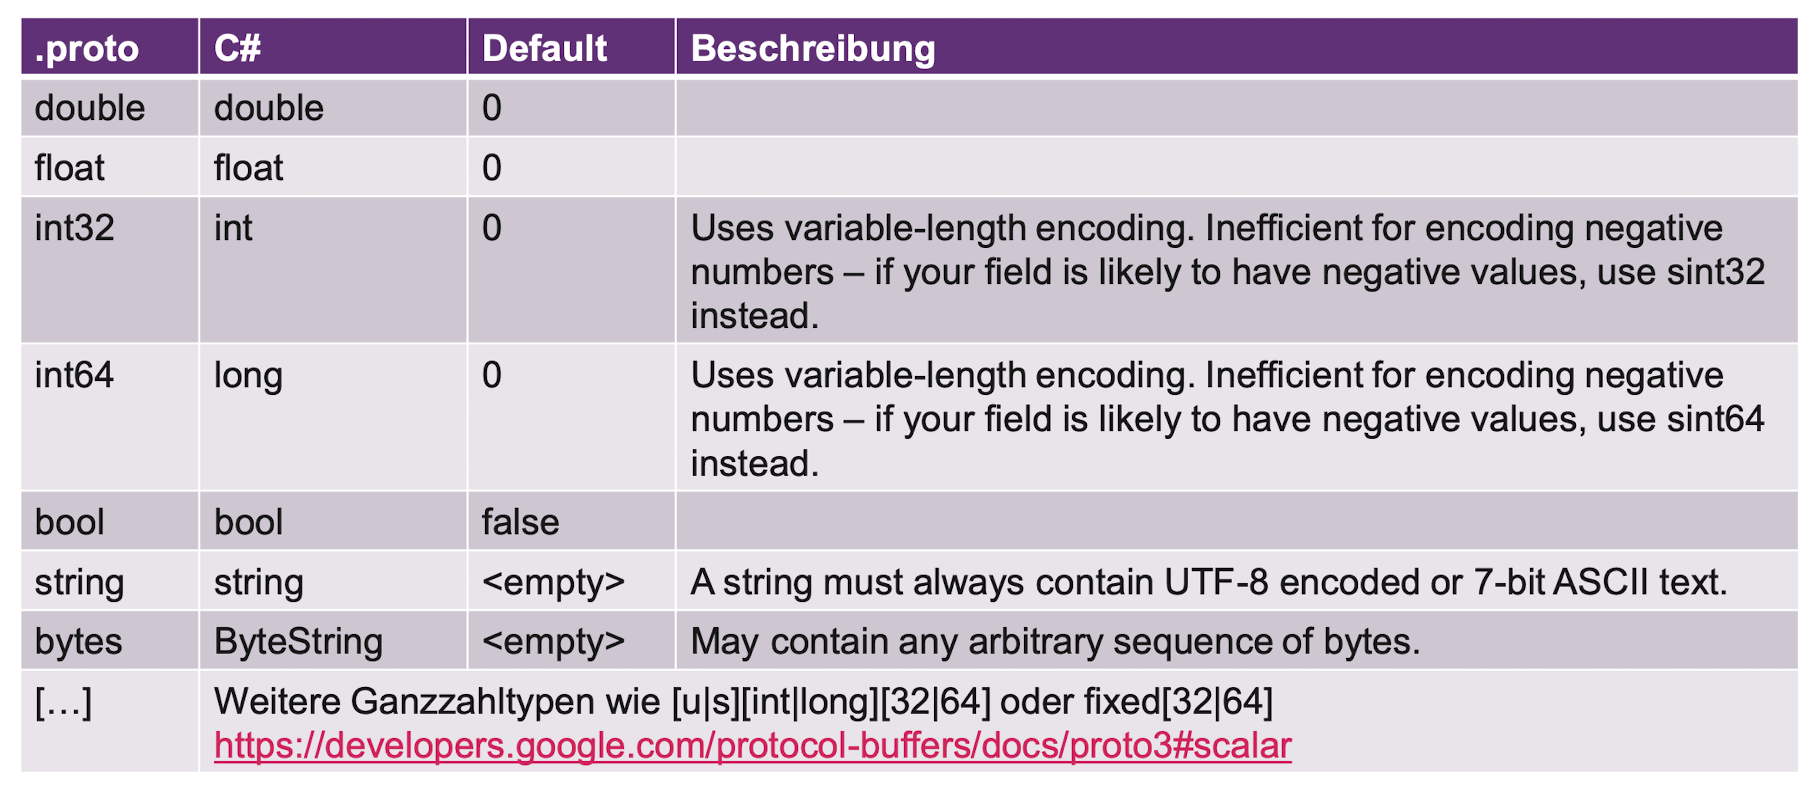
\includegraphics[width=0.75\linewidth]{protodatatypes}
  \caption{Felder Datentypen}
\end{figure}

\textbf{Proto Files}
\begin{lstlisting}
syntax = "proto3"; 
option csharp_namespace = "_01_BasicExample"; 
package Greet; 

// The greeting service definition. 
service Greeter {
  rpc SayHello (HelloRequest) returns (HelloReply);
} 

// The request message containing the user's name. 
message HelloRequest {
  string name = 1; 
} 
// The response message containing the greetings. 
message HelloReply {
  string message = 1; 
}
\end{lstlisting}

\textbf{Fields/Repeated Fields} \\
\begin{itemize}
    \item \textbf{Angabe des Feldtypen} Skalarer Werttyp, andere Message Type, Enumeration
    \item \textbf{Unique Field Name} Wird für Generatoren verwendet, Lower Snake Case (underscores)
    \item \textbf{Unique Field Number} Identifikator für das Binärformat.
\end{itemize}
\begin{lstlisting}
message SearchRequest {
	string query = 1;
	int32 page_number = 2;
	int32 result_per_page = 3; 
}
message SearchResponse {
	repeated string results = 1; // Repeated = Liste
}
\end{lstlisting}

\textbf{Enumerations}\\
Von  der Idee her analog zu Enumerationstypen (enum) in .NET. Enum-Member mit dem Wert 0 muss zwingend existieren.
\begin{lstlisting}
message SearchRequest {
	Color searchColor = 1;
	Size searchSize = 2;
	enum Color {
		RED = 0; // 0 must exist 
		GREEN = 1;
	}
} 
enum Size {
	S = 0; // 0 must exist
	M = 1;
	L = 2; 
}	
\end{lstlisting} 

\textbf{Reserved Fields}\\
Für Versionierung gedacht. Wiederverwendung wird vom Protocol Buffer Compiler verhindert. 
\begin{lstlisting}
message SearchRequest {
	reserved 1, 3, 20 to 30;
	reserved "page_number", "result_per_page"; 
	string query = 1; // Compilerfehler
	int32 page_number = 2; // Compilerfehler 
	int32 result_per_page = 3; // Compilerfehler
}
\end{lstlisting}

\subsection{gRPC \# API}
\textbf{Protocol Buffer Compiler}
\begin{itemize}
	\item protoc.exe mit Plugin für C\# Code Generierung
	\item Automatische in Build Pipeline eingebunden
	\item NuGet Package: grpc.Tools
	\item Proto-Compiler Ouput in "obj" order
\end{itemize}

\subsection{Beispiel Customer Service}
Zwei Services Customer und Order Service.

\textbf{Customer Service}
\begin{lstlisting}
service CustomerService {
  rpc GetCustomers (google.protobuf.Empty)
    returns (GetCustomersResponse);
  rpc GetCustomer (GetCustomerRequest) 
    returns (GetCustomerResponse);
}
\end{lstlisting}

\textbf{Order Service}
\begin{lstlisting}
service OrderService {
	rpc GetOrders (GetOrdersRequest) 
	returns (GetOrdersResponse);
}
\end{lstlisting}

\textbf{Service Implementation} \\
\begin{lstlisting}
//Customer Service
public class MyCustomerService : CustomerService.CustomerServiceBase {
    public override async Task<GetCustomersResponse> GetCustomers(Empty request, ServerCallContext context) { /* ... */ }
    public override async Task<GetCustomerResponse> GetCustomer(GetCustomerRequest request, ServerCallContext context) { /* ... */ }
}

//Order Service
public class MyOrderService : OrderService.OrderServiceBase {
    public override async Task<GetOrdersResponse> GetOrders(GetOrdersRequest request, ServerCallContext context) { /* ... */ }
}
\end{lstlisting}

\textbf{Client-Implementation (Customer)}
\begin{lstlisting}
// The port number (5001) must match the port of the gRPC server.
GrpcChannel channel = GrpcChannel.ForAddress("https://localhost:5001");

// Customer service calls
var customerClient = new CustomerService.CustomerServiceClient(channel);

var request1 = new Empty();
GetCustomersResponse response1 = await customerClient.GetCustomersAsync(request1);
Console.WriteLine(response1);

var request2 = new GetCustomerRequest { IdFilter = 1 };
GetCustomerResponse response2 = await customerClient.GetCustomerAsync(request2);
Console.WriteLine(response2);

request2.IncludeOrders = false;
response2 = await customerClient.GetCustomerAsync(request2);
Console.WriteLine(response2);
\end{lstlisting}

\textbf{Client-Implementation (Order)}
\begin{lstlisting}
// The port number (5001) must match the port of the gRPC server.
GrpcChannel channel = GrpcChannel.ForAddress("https://localhost:5001");

// Order service calls
var orderClient = new OrderService.OrderServiceClient(channel);

var request3 = new GetOrdersRequest { CustomerIdFilter = 1 };
GetOrdersResponse response3 = await orderClient.GetOrdersAsync(request3);
Console.WriteLine(response3);
\end{lstlisting}


\subsection{Streams}
Es werden \textbf{drei Modi} unterstüzt: Server Streaming (Sever - Client), Client Streaming (Client - Server), Bi-directional / Duplex Streaming Call. Es werden zwei verschiedene Modi von Lesen unterstützt: Synchrones und asynchrones lesen. \textbf{Reliability} End-to-End Reliability (garantiertes Ausliefern der Nachrichten gewährleistet), Ordered Delivery (Reihenfolge gewährleistet).

\begin{lstlisting}
service FileStreamingService {
  rpc ReadFiles (google.protobuf.Empty)
    returns (stream FileDto);
  rpc SendFiles (stream FileDto)
    returns (google.protobuf.Empty);
  rpc RoundtripFiles (stream FileDto) 
    returns (stream FileDto);
}
message FileDto {
  string file_name = 1;
  int32 line = 2;
  string content = 3; 
}
\end{lstlisting}

\subsection{Exception Handling}
Grundsätzlich immer via ”RpcException” (basierend auf StatusCodes).
\begin{lstlisting}
public class RpcException : Exception {
    public RpcException(Status status);
    public RpcException(Status status, string message);
    public RpcException(Status status, Metadata trailers);
    public RpcException(Status status, Metadata trailers, string message);
    public Status Status { get; }
    public StatusCode StatusCode { get; }
    public Metadata Trailers { get; }
}
\end{lstlisting}

\begin{figure}[h!]
  \center
  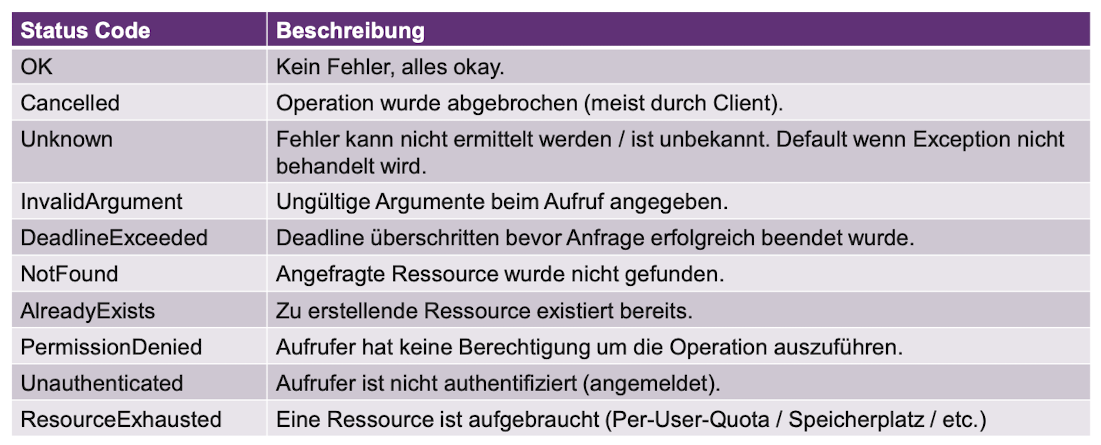
\includegraphics[width=0.49\linewidth]{grpcstatus1}
  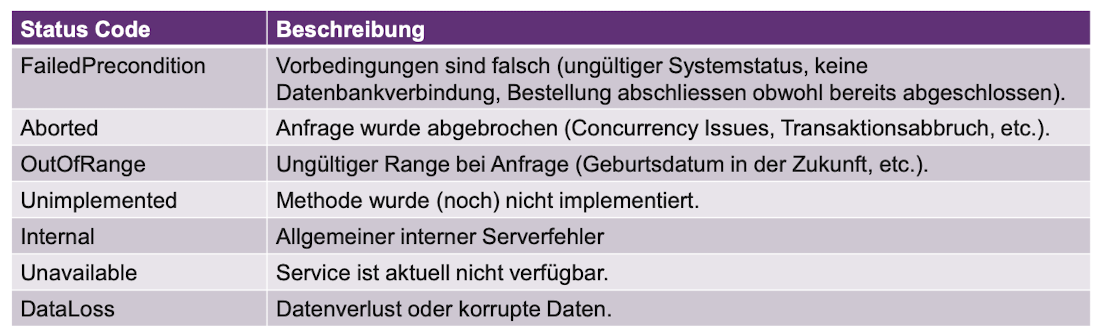
\includegraphics[width=0.49\linewidth]{grpcstatus2}
\end{figure}

\textbf{Unbehandelte Exception} \\
Exception wird auf Server nicht gefangen (Server Runtime fängt Exception, Wirft RpcException)
\begin{lstlisting}
public override async Task<Empty> Unhandled(Empty request, ServerCallContext context) {
    throw new Exception("Unhandled Exception");
}
\end{lstlisting}

\textbf{Behandelte Exception mit Trailers} \\
Exception wird auf Server gefangen und korrekt verpackt. Metadata-Klassen verwenden, Key-Value-Pair-Liste.
\begin{lstlisting}
public override async Task<Empty> Trailers(Empty request, ServerCallContext context) {
    throw new RpcException(new Status(StatusCode.NotFound, "Something was not found."),
        new Metadata {
            { "error-details", "Here are some more details..." },
            { "error-obj" + Metadata.BinaryHeaderSuffix, Encoding.UTF8.GetBytes("...payload...") }
        }
    );
}
\end{lstlisting}

\pagebreak